\documentclass{article}
\usepackage[utf8]{inputenc}
\usepackage{graphicx}
\usepackage{geometry}
\usepackage{hyperref}
\usepackage{float}
\hypersetup{
    colorlinks,
    citecolor=black,
    filecolor=black,
    linkcolor=black,
    urlcolor=black
}

 \geometry{
 a4paper,
 left=30mm,
 right=30mm,
 top=30mm,
 }

\graphicspath{ {Images/} }

%----------------------------------------------------------------------------------------
%	TITLE PAGE
%----------------------------------------------------------------------------------------

\newcommand*{\titleGP}{\begingroup
		\begin{figure}[t]
			\centering
			
\includegraphics[width=350px]{UP_Logo.PNG}
		\end{figure}		
\centering 
\vspace*{\baselineskip}

\rule{\textwidth}{1.6pt}\vspace*{-\baselineskip}\vspace*{2pt}
\rule{\textwidth}{0.4pt}\\[\baselineskip]

{\Huge Vulknut Software Engineering } \\ [0.2\baselineskip]
\rule{\textwidth}{0.4pt}\vspace*{-\baselineskip}\vspace{3.2pt}
\rule{\textwidth}{1.6pt}\\[\baselineskip] %

% \scshape %
% A concise specification on the functional requirements  \\
% and use cases of NavUP \\[\baselineskip]

% \vspace*{2\baselineskip}

\bigskip

Compiled By \\[\baselineskip]

\bigskip

{\Large Peter Boxall - u14056136 \\ Claude Greeff - u13153740 \\ Marin Peroski -  u13242475 \\ Johan du Plooy - u12070794 \\ Bernhard Shuld - u \\\par}

\bigskip
\bigskip
\bigskip
 
 	{\huge GitHub Repository:  
 	\href{https://github.com/Valknut-Software-Engineering/Capstone_Project}{Valknut Software Engineering}\par}
 		 	
\bigskip
\bigskip
\bigskip

	\begin{figure}[H]
			\centering
			
\includegraphics[width=200px,height=125px]{epiUse.PNG}
	\end{figure}
	
\vfill

{\Large 2017} \\[0.3\baselineskip]

\endgroup}

\begin{document}

\titleGP
\newpage
\tableofcontents
\newpage

\section{Introduction}

	\subsection{Purpose}
	This document serves to outline the overall description and requirements of 	the system. This document also serves as a guideline to the developers in 		order to ensure the final product meets these requirements, and indicates 		to the client what the required technologies are in order to be able to use 	this system.
	
	\subsection{Scope}
	
	Blah blah	
	
	\subsection{Definitions, Acronyms, and Abbreviations}
			\paragraph{MEAN}	MongoDB, Express.js, AngularJS (or Angular), and Node.js
			\paragraph{VR}	Virtual Reality
		% \section{References}

\section{Design}

	\subsection{Software Methodology}
	We will follow the Agile development methodology. The principles this methodology is based on advocates planning, constantly evolving development, early delivery and continues improvements, and it encourages flexibility as well as maintainability.
	
	\begin{flushleft}
	The agile development process is built on four main principles:
		\begin{enumerate}
			\item Individual and team interactions over processes and tools.
			\item Working software over comprehensive documentation.
			\item Customer collaboration over contract negotiation.
			\item Responding to change over following a plan.		
		\end{enumerate}	
	\end{flushleft}	
	
\begin{flushleft}		
Due to frequent meetings with the client we are preparing for numerous requirement changes to be made in which the agile methodology thrives in. Requirements, implementation, design, etc., are continually revisited through the agile development life cycle.

\bigskip

For these reasons we specifically chose agile software development as it is well-known and the most applicable.
\end{flushleft}

	\begin{figure}[H]
			\centering
			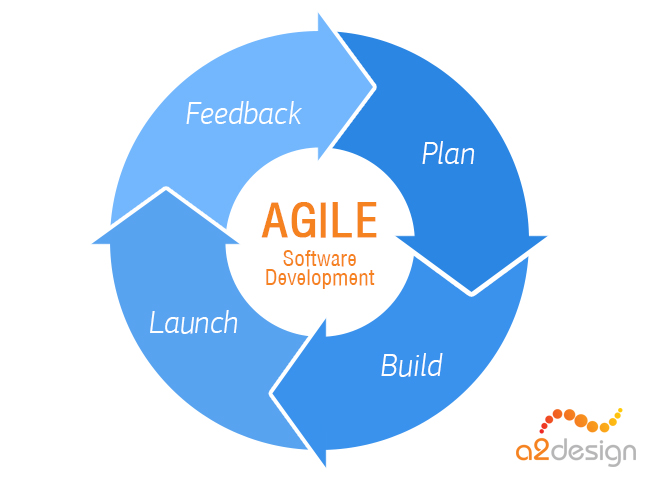
\includegraphics[width=200px,height=150px]{agile.JPG}
	\end{figure}
	
\section{System Requirements}

	\subsection{Functional Requirements}
	
	The following functional requirements will be met:
	
	\begin{enumerate}
			\item blah blah
	\end{enumerate}
	
	\subsection{Non-Functional Requirements}
	
	The following non-functional requirements will be met:
	
	\begin{enumerate}
			\item blah blah
	\end{enumerate}
	
\section{Target Audience Characteristics}
	
	blah blah education blah

\section{Technologies}
	\begin{enumerate}
		\item Creating a 3D environment to create a presentation.
		\item Unity 3D virtual reality system tool kit library.
		\item HTC Vive virtual reality gear (already available).
		\item Import external models.
		\item Windows 10 environment.
		\item Docker.
		\item TravisCI.	
	\end{enumerate}
	

\end{document}